% !TEX root = ../main.tex
% Бүлэг 4

\chapter{Өгөгдөл боловсруулалт}
\label{Chapter4}
\pagecolor{Beige}

%-------------------------------------------------------------------------------

\section{Өгөгдлийн эх сурвалж ба зөвшөөрөл}

Судалгаанд нийтэд нээлттэй зургаан рентген зургийн өгөгдлийн сан болон эдгэрэлтийн таамаглалд зориулсан нэг синтетик клиникийн өгөгдлийг ашигласан. Эдгээр эх сурвалжуудыг сонгохдоо судалгааны зориулалтаар ашиглах боломж, лицензийн тодорхой байдал, өвчтөний мэдээлэл нэргүйжүүлэгдсэн эсэх, мөн тухайн өгөгдөл нь ангилал, сегментчлэл, хугарлын зэрэг болон эдгэрэлтийн таамаглалын аль даалгаварт тохирохыг харгалзав.

MURA өгөгдлийн сан нь яс-булчингийн рентген зургаар баялаг бөгөөд эхний хоёр туршилтад хэвийн болон гажигтай дүрсийг ялгах ангиллын суурь өгөгдөл болсон~\cite{ref39}. Харин эцсийн модульчлагдсан pipeline-д MURA-г шууд сургалтын өгөгдөл болгон ашиглаагүй. FracAtlas нь хугарлын тодорхой жишээ, COCO форматтай маск болон хугарлын мета-өгөгдөл агуулдаг тул сегментчлэл болон хугарлын зэргийн үнэлгээнд гол эх сурвалж болж ашиглагдсан~\cite{ref40}. GRAZPEDWRI-DX нь хүүхдийн бугуйн рентген зураг, YOLO тэмдэглэгээ болон нас, хүйсийн мэдээлэл агуулдаг тул Туршилт 3-ын ангиллын өгөгдлийн үндсэн эх сурвалжуудын нэг болсон~\cite{ref41}.

Туршилт 3-ын ангиллын модульд GRAZPEDWRI-DX, FracAtlas-COCO, YOLOBoneFracture болон BoneFractureCVProject өгөгдлийн сангуудыг ашигласан. YOLO хайрцаг тэмдэглэгээтэй өгөгдлүүдийг Туршилт 3-ыг эхлүүлэхээс өмнөх өгөгдөл бэлтгэлийн шатанд SAM загварт prompt болгон дамжуулж, сегментчлэлийн псевдо масктай жишээ үүсгэхэд хэрэглэсэн. Эдгэрэлтийн бодит хугацааны урт хугацааны тэмдэглэгээ нээлттэй өгөгдлийн сангуудад байхгүй байсан тул синтетик клиникийн өгөгдлийг зөвхөн proof-of-concept түвшинд ашигласан.

\begin{table}[H]
    \centering
    \caption{Судалгаанд ашигласан өгөгдлийн эх сурвалжууд}
    \label{tab:dataset_sources}
    \scriptsize
    \begin{tabularx}{\textwidth}{@{}>{\raggedright\arraybackslash}p{2.15cm}
        >{\raggedright\arraybackslash}p{1.55cm}
        >{\raggedright\arraybackslash}p{2.35cm}
        >{\raggedright\arraybackslash}X
        >{\raggedright\arraybackslash}p{1.65cm}@{}}
    \toprule
    \textbf{Өгөгдөл} & \textbf{Хэмжээ} & \textbf{Тэмдэглэгээ} & \textbf{Ашигласан зорилго} & \textbf{Лиценз} \\
    \midrule
    MURA & $\sim$40,000 зураг & Normal/ abnormal & Туршилт 1--2-ын ангиллын суурь өгөгдөл & Судалгааны зориулалт \\
    FracAtlas & 4,083 зураг & Binary, COCO mask & Сегментчлэл, хугарлын зэрэг & CC BY 4.0 \\
    \shortstack[l]{GRAZPEDWRI\\-DX} & 20,327 зураг & YOLO bbox, нас/хүйс & Туршилт 3-ын ангилал & CC BY 4.0 \\
    \shortstack[l]{FracAtlas\\-COCO} & 966 зураг & COCO JSON & Туршилт 3-ын ангилал & CC BY 4.0 \\
    \shortstack[l]{YOLOBone\\Fracture} & 3,979 зураг & YOLO bbox & Туршилт 3-ын ангилал, псевдо маск бэлтгэл & CC0 \\
    \shortstack[l]{BoneFracture\\CVProject} & 3,631 зураг & YOLO bbox & Туршилт 3-ын ангилал, псевдо маск бэлтгэл & CC BY 4.0 \\
    Синтетик өгөгдөл & 5,000 мөр & Клиникийн хувьсагч & Эдгэрэлтийн таамаглал & Зохиомол \\
    \bottomrule
    \end{tabularx}
\end{table}

Бүх рентген зургийн өгөгдөл нь нийтэд нээлттэй хэлбэрээр түгээгдсэн бөгөөд өвчтөний шууд таних мэдээлэл агуулаагүй. Гэсэн хэдий ч өгөгдөл бүрийн лиценз, эх сурвалжийн нөхцөлийг хүндэтгэн зөвхөн судалгааны болон туршилтын зорилгоор ашиглав. Синтетик өгөгдөл нь бодит өвчтөний мэдээлэл агуулаагүй тул хувийн нууцын шууд эрсдэл бага боловч бодит клиникийн өгөгдлийг бүрэн төлөөлөхгүй гэсэн хязгаарлалтыг үр дүнгийн тайлбарт харгалзан үзсэн.

%-------------------------------------------------------------------------------

\section{Урьдчилсан боловсруулалт ба өгөгдөл нэмэгдүүлэлт}

Өгөгдлийн сангууд нь өөр өөр эх сурвалжаас бүрдсэн тул дүрсний хэмжээ, формат, суваг, тодрол, тэмдэглэгээний хэлбэр харилцан адилгүй байв. Иймээс сургалтад оруулахын өмнө дүрс бүрийг нэгэн ижил pipeline-аар боловсруулж, загварын оролтын шаардлагад нийцүүлсэн.

\subsection*{Дүрсний урьдчилсан боловсруулалт}

Эхний шатанд бүх зургийг уншиж, эвдэрсэн эсвэл дутуу файлыг хассан. Grayscale хэлбэртэй зургуудыг гурван сувагтай болгож, ImageNet дээр урьдчилан сургагдсан загваруудын оролтын хэлбэртэй нийцүүлэв. Ангиллын даалгаварт оролтын хэмжээг ихэвчлэн $224\times224$ болгосон бол сегментчлэлийн даалгаварт хугарлын нарийн шугамыг хадгалахын тулд $512\times512$ хэмжээг ашигласан.

Пикселийн утгыг $[0,255]$ завсраас $[0,1]$ завсарт хөрвүүлж, дараа нь ImageNet-ийн дундаж болон стандарт хазайлтаар нормчилсон. Энэ нь урьдчилан сургагдсан ConvNeXt, EfficientNet болон ResNet төрлийн загваруудыг ашиглах үед оролтын тархалтыг сургалтын эх тархалттай ойролцоо байлгах зорилготой.

\begin{equation}
    \hat{x} = \frac{x/255 - \mu_{\text{IN}}}{\sigma_{\text{IN}}}, \quad
    \mu_{\text{IN}} = [0.485,\ 0.456,\ 0.406], \quad
    \sigma_{\text{IN}} = [0.229,\ 0.224,\ 0.225]
\end{equation}

Дүрсний урьдчилсан боловсруулалтын үндсэн алхмуудыг (анхны зураг, хэмжээ өөрчлөлт, нормчлол) Зураг~\ref{fig:preprocess_steps}-д үзүүлэв.

\begin{figure}[H]
    \centering
    \begin{minipage}{0.31\textwidth}\centering
        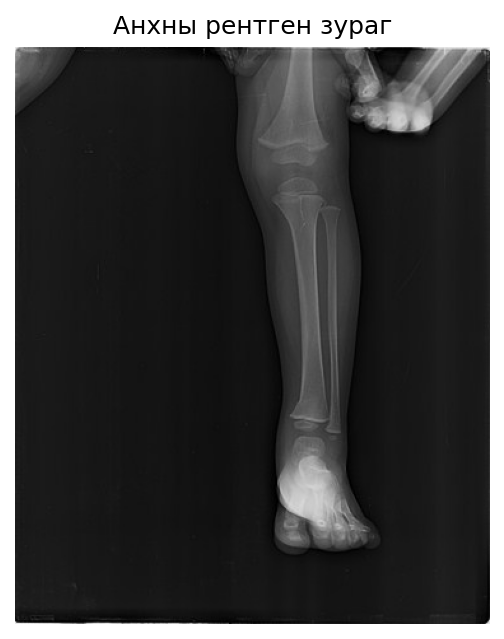
\includegraphics[width=\linewidth,height=0.26\textheight,keepaspectratio]{Figures/appx_b1_original.png}\\{\scriptsize (а) Анхны зураг}
    \end{minipage}\hfill
    \begin{minipage}{0.31\textwidth}\centering
        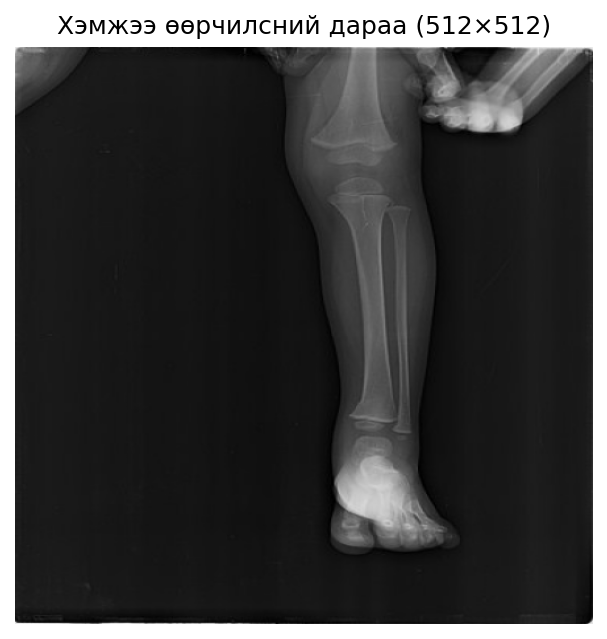
\includegraphics[width=\linewidth,height=0.26\textheight,keepaspectratio]{Figures/appx_b2_resized.png}\\{\scriptsize (б) Хэмжээ өөрчилсөн}
    \end{minipage}\hfill
    \begin{minipage}{0.31\textwidth}\centering
        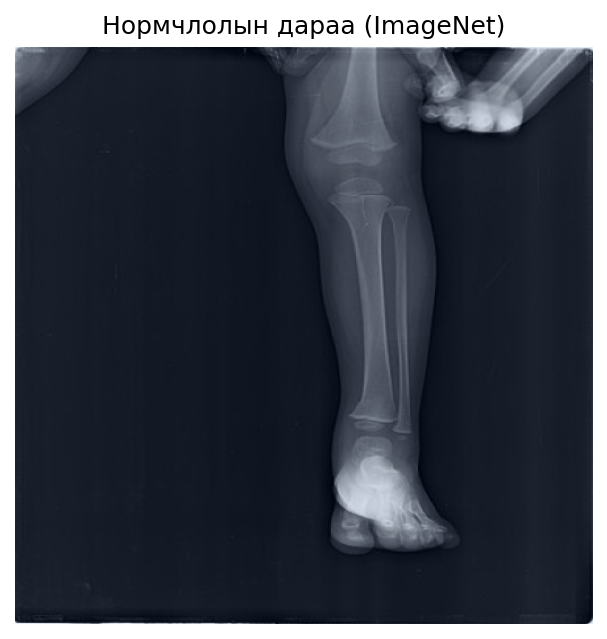
\includegraphics[width=\linewidth,height=0.26\textheight,keepaspectratio]{Figures/appx_b3_normalized.png}\\{\scriptsize (в) Нормчилсон}
    \end{minipage}
    \figcaption{Дүрсийн урьдчилсан боловсруулалтын алхмууд}{Дүрсийн урьдчилсан боловсруулалтын алхмууд: (а) анхны рентген зураг, (б) хэмжээ өөрчилсний дараах, (в) нормчлол хийсний дараах}
    \label{fig:preprocess_steps}
\end{figure}

FracAtlas-ийн COCO polygon тэмдэглэгээг хоёртын маск болгон хувиргасан. Маскийг resize хийхдээ nearest-neighbor interpolation хэрэглэсэн бөгөөд энэ нь маскийн 0 ба 1 утгын хоёртын шинжийг хадгалах давуу талтай. Харин рентген зургийн хэмжээг өөрчлөхөд bilinear interpolation ашигласан.

Туршилт 3-ыг эхлүүлэхээс өмнө YOLOBoneFracture болон BoneFractureCVProject өгөгдлийн сангийн YOLO хайрцаг тэмдэглэгээг SAM загварт prompt болгон өгч, хугарлын бүсийн псевдо маск үүсгэсэн. Энэ алхам нь эхний хоёр туршилтын сургалтад ашиглагдаагүй бөгөөд зөвхөн Туршилт 3-ын сегментчлэлийн өгөгдлийг өргөтгөх бэлтгэл ажил байсан. Үүссэн псевдо маскуудыг итгэлийн оноо, маскийн талбай, хоосон маск болон металл implant-ийн нөлөө зэрэг шалгуураар шүүж, чанарын шаардлага хангаагүй жишээг сургалтад оруулаагүй.

\subsection*{Мета-өгөгдөл ба шошго нэгтгэл}

Ангиллын даалгаварт эх сурвалж бүрийн шошгыг хугаралтай болон хугаралгүй гэсэн хоёртын хэлбэрт нэгтгэсэн. MURA-ийн abnormal шошго нь заавал хугарал гэсэн утгатай биш тул уг өгөгдлийг зөвхөн эхний хоёр туршилтад ерөнхий эмгэг өөрчлөлт ялгах суурь мэдлэг олгох зорилгоор ашигласан. Эцсийн ConvNeXt-Base ангилагчид GRAZPEDWRI-DX, FracAtlas-COCO, YOLOBoneFracture болон BoneFractureCVProject өгөгдлийг ашигласан бөгөөд эдгээр нь Туршилт 3-ын ангиллын сургалтын үндсэн эх сурвалж болсон.

Хугарлын зэргийн хувьд эх өгөгдөлд эмчийн бүрэн 0--3 шатлалтай шошго байхгүй тул FracAtlas-ийн маск болон түүнээс гарсан морфологийн шинжүүдийг ашигласан. Маскийн талбай, хэлбэр, чиглэл, хэсгийн тоо зэрэг шинжүүдээр хугарлын зэргийн прокси мэдээлэл үүсгэсэн бөгөөд энэ нь клиникийн эцсийн үнэлгээг орлохгүй, зөвхөн дүрслэлийн хэмжигдэхүйц шинжид суурилсан proof-of-concept үнэлгээ юм.

GRAZPEDWRI-DX-ийн файлын нэр болон мета-өгөгдлөөс нас, хүйс зэрэг хувьсагчдыг ялган авч, эдгэрэлтийн таамаглалын оролтын нэг хэсэг болгон ашигласан. Эдгэрэлтийн хугацааны бодит шошго байхгүй тул эдгээр хувьсагчийг синтетик клиникийн өгөгдөлтэй хослуулан proof-of-concept түвшинд хэрэглэв.

\subsection*{Өгөгдөл нэмэгдүүлэлт}

Өгөгдөл нэмэгдүүлэлтийг зөвхөн сургалтын хуваалтад хэрэглэсэн. Баталгаажуулалт болон тестийн хуваалтад өгөгдөл нэмэгдүүлэх арга хэрэглэхгүй байж, загварын бодит ерөнхийлөх чадварыг хэмжих зарчим баримталсан. Нэмэлт хувиргалтуудыг сонгохдоо рентген зураг авах үеийн байрлал, тодрол, шуугиан болон аппаратын ялгааг дуурайх боломжтой эсэхийг харгалзсан.

\begin{table}[H]
    \centering
    \caption{Урьдчилсан боловсруулалт ба өгөгдөл нэмэгдүүлэлтийн нэгтгэл}
    \label{tab:preprocess_augmentation}
    \small
    \begin{tabular}{p{3.6cm} p{4.4cm} p{4.4cm}}
    \toprule
    \textbf{Алхам} & \textbf{Арга} & \textbf{Зорилго} \\
    \midrule
    Хэмжээ нэгтгэх & $224\times224$ ангилал, $512\times512$ сегментчлэл & Загварын оролтыг стандартчилах \\
    Суваг нэгтгэх & Grayscale зургийг 3 сувагт хөрвүүлэх & Урьдчилан сургагдсан загварт нийцүүлэх \\
    Нормчлол & ImageNet mean/std & Оролтын тархалтыг тогтворжуулах \\
    Маск хөрвүүлэх & COCO polygon $\rightarrow$ binary mask & Сегментчлэлийн ground truth бэлтгэх \\
    CLAHE & Орон нутгийн контраст нэмэгдүүлэх & Хугарлын нарийн шугамыг тодруулах \\
    Геометрийн хувиргалт & Эргүүлэлт, тусгал, тайралт & Байрлалын хэлбэлзэлд тэсвэртэй болгох \\
    Пикселийн хувиргалт & Тодрол, контраст, Gaussian noise & Дүрсний чанарын хэлбэлзлийг дуурайх \\
    Mixup~\cite{zhang2018mixup} & $\alpha=0.2$ & Ангиллын ерөнхийлөх чадварыг нэмэгдүүлэх \\
    \bottomrule
    \end{tabular}
\end{table}

Сегментчлэлийн даалгаварт зураг болон масктай холбоотой геометрийн хувиргалтыг ижил параметрээр хэрэглэсэн. Харин тодрол, контраст, шуугиан зэрэг пикселийн түвшний хувиргалтыг зөвхөн зурагт хэрэглэж, маскийг өөрчлөөгүй. Энэ нь хугарлын байрлалын шошгыг зөрүүлэхгүй байх шаардлагатай холбоотой. Сургалтын хуваалтад хэрэглэсэн өгөгдөл нэмэгдүүлэлтийн жишээг Зураг~\ref{fig:augment_example}-д үзүүлэв.

\begin{figure}[H]
    \centering
    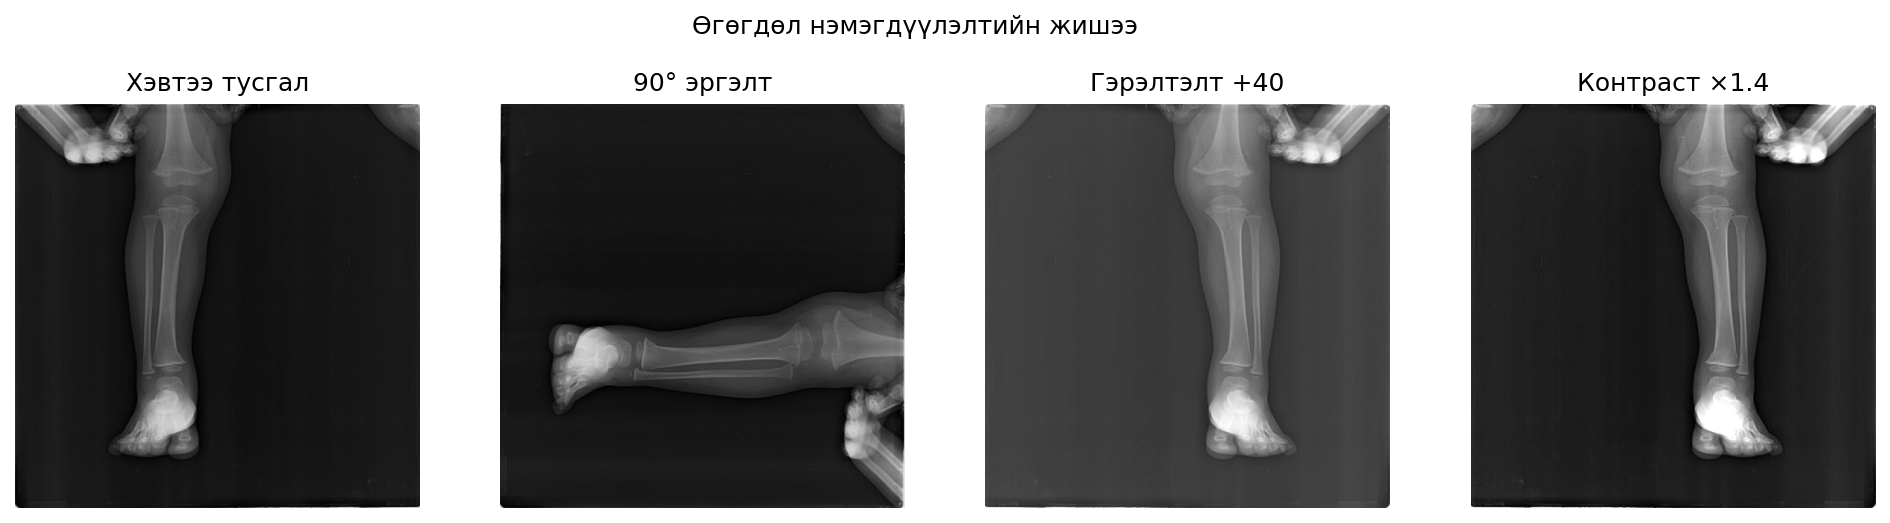
\includegraphics[width=0.85\textwidth,height=0.34\textheight,keepaspectratio]{Figures/appx_b4_augment.png}
    \figcaption{Өгөгдөл нэмэгдүүлэлтийн жишээ}{Сургалтын хуваалтад хэрэглэсэн өгөгдөл нэмэгдүүлэлтийн жишээ}
    \label{fig:augment_example}
\end{figure}

%-------------------------------------------------------------------------------

\section{Train/validation/test хуваалт}

Загварын гүйцэтгэлийг бодитой үнэлэхийн тулд өгөгдлийг сургалт, баталгаажуулалт, тестийн гурван хэсэгт хуваасан. Сургалтын хэсгийг загварын параметр сурахад, баталгаажуулалтын хэсгийг гиперпараметр болон босго утга сонгоход, тестийн хэсгийг зөвхөн эцсийн гүйцэтгэлийг хэмжихэд ашигласан. Ингэснээр тестийн мэдээлэл сургалтын явцад урьдчилан нөлөөлөхөөс сэргийлсэн. Хүснэгт~\ref{tab:data_split}-д өгөгдлийн сан бүрт баримталсан ойролцоох хуваалтын зарчмыг нэгтгэн үзүүлэв.

Хуваалт хийхдээ боломжтой тохиолдолд ангийн харьцааг хадгалах stratified split ашигласан. Нэг өвчтөн эсвэл нэг судалгаанд хамаарах олон зураг байвал нэг хуваалтад хамтад нь байлгах зарчим баримталсан. Энэ нь ижил өвчтөний ойролцоо зураг train болон test-д зэрэг орох data leakage-ийн эрсдэлийг бууруулна. Дахин давтагдах чадварыг хангахын тулд санамсаргүй хуваалт хийх үед тогтмол seed ашигласан.

\begin{table}[H]
    \centering
    \caption{Өгөгдлийн хуваалтын ерөнхий зарчим}
    \label{tab:data_split}
    \small
    \begin{tabular}{p{3.1cm} p{2.2cm} p{2.2cm} p{2.2cm} p{3.3cm}}
    \toprule
    \textbf{Өгөгдөл} & \textbf{Train} & \textbf{Validation} & \textbf{Test} & \textbf{Тэмдэглэл} \\
    \midrule
    MURA & 70--80\% & 10--15\% & 10--15\% & Туршилт 1--2-ын ангиллын суурь сургалт \\
    FracAtlas & 70--80\% & 10--15\% & 10--15\% & Масктай хэсгийг сегментчлэлд ашигласан \\
    \shortstack[l]{GRAZPEDWRI\\-DX} & 70--80\% & 10--15\% & 10--15\% & Нас, хүйсийн хувьсагч ялгасан \\
    \shortstack[l]{FracAtlas\\-COCO} & 70\% & 15\% & 15\% & Туршилт 3-ын ангилал \\
    \shortstack[l]{YOLOBone\\Fracture} & 70\% & 15\% & 15\% & Туршилт 3-ын ангилал, псевдо маск бэлтгэл \\
    \shortstack[l]{BoneFracture\\CVProject} & 70\% & 15\% & 15\% & Туршилт 3-ын ангилал, псевдо маск бэлтгэл \\
    Синтетик өгөгдөл & 80\% & 10\% & 10\% & Эдгэрэлтийн туршилтын модуль \\
    \bottomrule
    \end{tabular}
\end{table}

Эхний хоёр туршилтад MURA өгөгдлийг ангиллын суурь сургалтад ашигласан. Харин эцсийн ConvNeXt-Base ангилагчийн сургалтад GRAZPEDWRI-DX, FracAtlas-COCO, YOLOBoneFracture болон BoneFractureCVProject өгөгдлийг нэгтгэн нийт 28,903 зураг ашигласан. Нэгдсэн өгөгдөлд хугаралтай болон хэвийн жишээний харьцаа тэнцвэргүй байсан тул сургалтын үед WeightedRandomSampler болон Focal BCE алдагдлыг ашиглаж ангийн тэнцвэргүй байдлын нөлөөг багасгасан.

\begin{table}[H]
    \centering
    \caption{Эцсийн ConvNeXt-Base ангилагчид ашигласан нэгдсэн өгөгдлийн хуваалт}
    \label{tab:v2_combined}
    \small
    \begin{tabular}{p{3.4cm} r r r r}
    \toprule
    \textbf{Өгөгдөл} & \textbf{Нийт} & \textbf{Train} & \textbf{Validation} & \textbf{Test} \\
    \midrule
    \shortstack[l]{GRAZPEDWRI\\-DX} & 20,327 & 14,228 & 3,049 & 3,050 \\
    \shortstack[l]{FracAtlas\\-COCO} & 966 & 676 & 145 & 145 \\
    \shortstack[l]{YOLOBone\\Fracture} & 3,979 & 2,785 & 597 & 597 \\
    \shortstack[l]{BoneFracture\\CVProject} & 3,631 & 2,542 & 544 & 545 \\
    \midrule
    \textbf{Нийт} & \textbf{28,903} & \textbf{20,231} & \textbf{4,335} & \textbf{4,337} \\
    \bottomrule
    \end{tabular}
\end{table}

Туршилт 3-ын сегментчлэлийн сургалтад FracAtlas-ийн гараар тэмдэглэсэн маскуудаас гадна өмнөх бэлтгэл шатанд SAM-аар үүсгэсэн псевдо маскуудыг нэмж хэрэглэсэн. Эдгээр псевдо шошго нь эмчийн гараар баталгаажуулсан масктай адил түвшний найдвартай биш гэдгийг үр дүнгийн тайлбарт харгалзсан.

%-------------------------------------------------------------------------------

\section{Чанарын үзүүлэлтийн хүснэгт}

Өгөгдлийн чанарыг шалгахдаа техникийн бүрэн бүтэн байдал, шошгоны нийцэл, ангийн тархалт болон псевдо шошгоны найдвартай байдлыг тусад нь авч үзсэн. Энэ шалгалт нь сургалтын явцад загвар буруу файл, хоосон маск, давхардсан зураг эсвэл буруу шошгоноос суралцах эрсдэлийг багасгах зорилготой.

\begin{table}[H]
    \centering
    \caption{Өгөгдлийн чанарын шалгалтын үзүүлэлтүүд}
    \label{tab:quality_indicators}
    \small
    \begin{tabular}{p{3.6cm} p{4.8cm} p{4.0cm}}
    \toprule
    \textbf{Үзүүлэлт} & \textbf{Шалгах арга} & \textbf{Хэрэгжүүлсэн шийдэл} \\
    \midrule
    Файлын бүрэн бүтэн байдал & PIL/OpenCV ашиглан зураг нээгдэх эсэхийг шалгах & Эвдэрсэн болон уншигдахгүй файлыг хасах \\
    Давхардал & Файлын hash болон замын давхардлыг шалгах & Давхардсан жишээг сургалтаас гаргах \\
    Шошгоны нийцэл & CSV, JSON, YOLO label болон файлын нэрийг тулгах & Тохирохгүй мөрийг засах эсвэл хасах \\
    Маскийн чанар & Маскийн пикселийн нийлбэр, талбайн хувь, polygon цэгийн тоо & Хоосон болон хэт том/жижиг маскийг шүүх \\
    Псевдо маск & SAM confidence score, bbox болон маскийн давхцал & Итгэл багатай псевдо шошгыг ашиглахгүй байх \\
    Ангийн тэнцвэргүй байдал & Хугаралтай/хэвийн жишээний харьцаа тооцох & Weighted sampling, Focal loss хэрэглэх \\
    Нуугдмал системийн файл & macOS \texttt{.\_*} болон хэрэггүй metadata файл шалгах & Уншилтын алдаа үүсгэх файлыг шүүх \\
    \bottomrule
    \end{tabular}
\end{table}

\begin{table}[H]
    \centering
    \caption{Ангиудын тэнцвэргүй байдлын нэгтгэл}
    \label{tab:class_balance}
    \small
    \begin{tabular}{p{3.2cm} p{3.2cm} p{3.0cm} p{3.5cm}}
    \toprule
    \textbf{Өгөгдөл} & \textbf{Эерэг жишээ} & \textbf{Сөрөг жишээ} & \textbf{Ашигласан зохицуулалт} \\
    \midrule
    MURA & Abnormal зураг & Normal зураг & Туршилт 1--2-д class weighting \\
    FracAtlas & Хугаралтай зураг & Хугаралгүй зураг & Focal/Dice loss, sampling \\
    Эцсийн ангиллын өгөгдөл & Эх сурвалжаас хамаарсан & Эх сурвалжаас хамаарсан & WeightedRandomSampler + Focal BCE \\
    Хугарлын зэрэг & Grade 1--3 цөөн & Grade 0 давамгай & Морфологийн шинж, жинлэлт \\
    \bottomrule
    \end{tabular}
\end{table}

Чанарын шалгалтын дараа ч өгөгдлийн гарал үүсэлтэй холбоотой хэд хэдэн хязгаарлалт үлдэнэ. MURA-ийн abnormal шошго нь зөвхөн хугарлыг илэрхийлэхгүй, бусад яс-булчингийн өөрчлөлтийг хамардаг тул уг өгөгдлийг зөвхөн эхний хоёр туршилтын суурь ангиллын сургалтад ашигласан. FracAtlas-ийн хугарлын зэргийн бүрэн клиникийн шошго байхгүй тул морфологийн шинжид суурилсан прокси үнэлгээ ашигласан. Туршилт 3-ын өмнөх бэлтгэл шатанд SAM-аар үүсгэсэн псевдо маск нь гараар баталгаажуулсан шошго биш тул сегментчлэлийн үр дүнд тодорхой хэмжээгээр нөлөөлөх боломжтой. Эдгээр хязгаарлалтыг \ref{Chapter6}~бүлгийн үр дүнгийн хэлэлцүүлэг болон \ref{Chapter7}~бүлгийн ёс зүйн үнэлгээнд харгалзан авч үзсэн.
